\chapter{Introducción}

\section{Introducción}
El objetivo de este proyecto es la creación de un software capaz de transformar de forma autonoma un modelo 3D detallado de una escultura cualquiera en una escultura que inmita el estilo del escultor Pablo Emilio Gargallo Catalán.
Este estilo se caracteriza principalmente por jugar con las concavidades y las convexidades de las esculturas para obtener efectos no obtenibles por medio de tecnicas tradicionales.

\begin{figure}
    \centering
    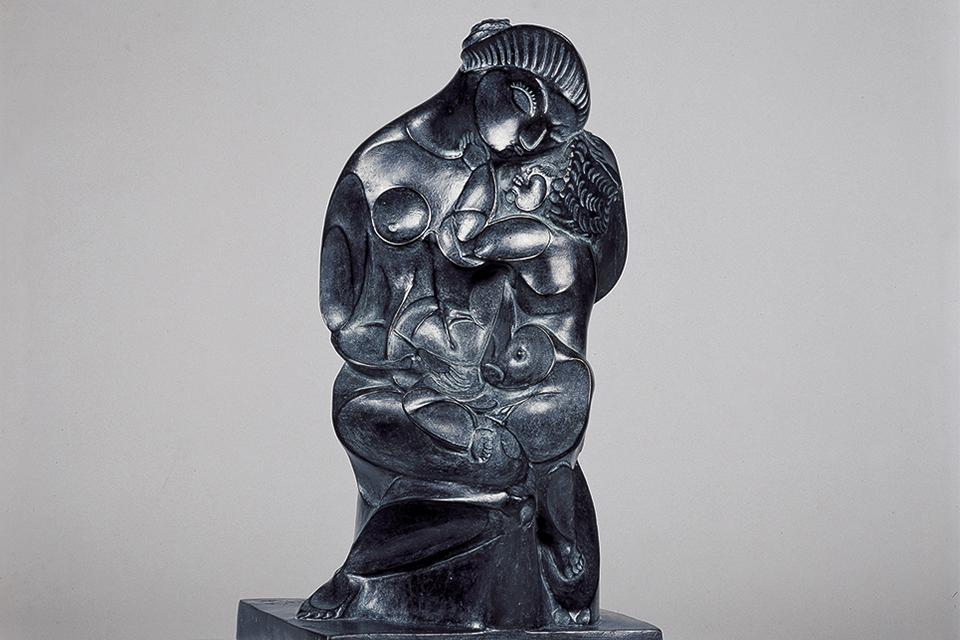
\includegraphics[width=\textwidth]{imagenes/maternidad_gargallo.jpg}
    \caption{Ejemplo de una escultura de Pablo Gargallo}
\end{figure}


Nuestro punto focal de interes va a ser precisamente lograr transformar las convexidades de los modelos 3D en concavidades. Para permitirnos hacer esto vamos a utilizar varios recursos de los graficos por ordenador.

\section{Los graficos por ordenador}
\subsection{Definicion de graficos por ordenador}
El termino graficos por ordenador se refiere a un campo multidisciplinar donde se agrupa cualquier disciplina que contribuye a la creación y visualización de representaciones pictoricas enteremante en un ordenador\cite{Foley_1995}.
Esto engloba una variedad de campos donde hay discusión sobre si pertenecen o no al ambito de los graficos por ordenador.Sin embargo hay 3 campos principales en los cuales hay consenso general de que forman parte de la disciplina.
\begin{list}{.}{}
    \item El modelado, que es la rama que lidia con la representación matematica de la especificación de la forma y la apariencia de una representación pictorica concreta de forma que sea interpetable para un ordenador
    \item El Renderizado, que lidia con la creación de las representaciones 2D finales de nuestros modelos 3D tras la aplicación de luces, texturas y materiales 
    \item La animación que es la tecnica para crear ilusión de movimiento a partir de la secuenciación de Imagenes. Dentro de esta rama se utilizan conceptos del renderizado y el modelado pero se le añade el factor clave del movimiento en el tiempo
\end{list} \cite{marschner_fundamentals_2018}

Para nuestro proyecto los campos relevantes son solo el modelado y el renderizado. Puesto que al final del proyecto nuestro objetivo es poder visualizar de forma dinamica esa escultura "Gargallizada" y ademas poder exportar una representación de la escultura luego de ser modificada para poder ser impresa en 3D.

La capacidad de poder visualizar los graficos por ordenador necesitamos generar una imagen sintetica en dos dimensiones que pueda ser representada sobre la pantalla del ordenador. Para ello se definen todos los elementos del entorno tridimensional, siendo esto no solo los modelos tridimensionales sino tambien la presencia de luces. Las cuales de hecho son obligatorias. Pues sin ellas todo se vería oscuro. 
En su defecto las API de graficos por ordenador utilizan una luz ambiente que aplica de igual forma a todos los elementos. Y finalmente el ultimo elemento necesario es una camara que nos permite crear un sentido de perspectiva y colocar un punto de referencia desde el cual se esta visualizando la escena.

Una vez todos los elementos estan definidos la API de graficos que vayamos a utilizar realizara una serie de operaciones para conseguir esa representacion pictorica bidimensional de nuestro modelo. Las cuales se ejecutan en GPU. Esta serie de operaciones es lo que conocemos como "pipeline" de graficos. Este pipeline de transformaciones dependera del proceso que utilice la API de graficos para generar
la imagen bidimensional final. En  nuestro caso para este trabajo estamos utilizando OpenGL, la cual es una API de graficos que utiliza rasterización para el renderizado. Pero existen otras alternativas que recientemente estan cobrando mas popularidad como el Ray Tracing. Como hemos mencionado previamente en este trabajo hemos decidido emplear OpenGL como API de graficos. Esto se debe principalmente a dos motivos. El primero es uno de familiaridad puesto que OpenGL es la API de graficos
que se enseña en el grado. Ademas de eso el segundo motivo es que OpenGL es la API mas extendida entre todas las alternatives libres y multiplatadorma. Y aunque tiene competidores directos como la API Direct3D estos son privativos. Cabe mencionar que existe un estandar alternativo a OpenGL mas moderno llamado Vulkan, el cual permite un mayor control sobre lo que ocurre en la tarjeta grafica y ofrece un mayor rendimiento. Sin embargo el punto donde las diferencias de rendimiento entre Vulkan y OpenGL 
se hace notable es en proyectos mucho mas ambiciosos como videojuegos triple A con graficos hiperrealistas. Para nuestro proyecto elegir una u otra es indiferente. Y por tanto decidimos utilizar la API que ya conociamos y teniamos cierta experiencia previa.

\subsection{El pipeline de graficos}

\subsubsection{El pipeline de graficos fijo}
Conociendo entonces que API de graficos vamos a utilizar podemos pasar a describir el pipeline de graficos que utiliza OpenGL. Originalmente
openGL ha utilizado un pipeline de graficos fijo. Esto quiere decir que una vez los datos de geometrias, camaras, luces, texturas que hayamos definido en el programa 
que se esta ejecutando en la CPU van a la GPU las transformaciones que van a sufrir ya estan predefinidas y tenemos un grado de control muy limitado sobre ellas. En el pipeline de graficos fijo
de OpenGl las fases son las siguientes

\begin{figure}
    \centering
    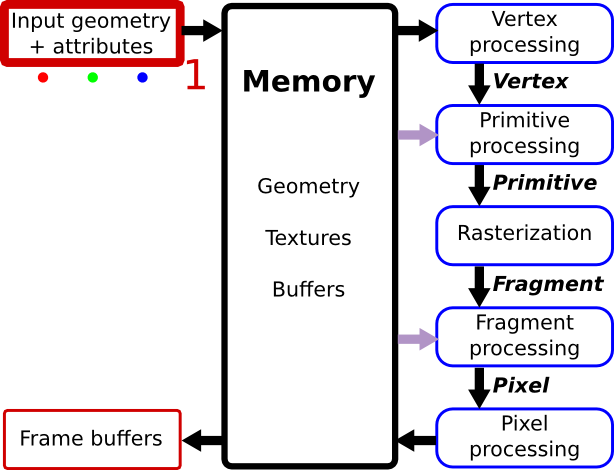
\includegraphics[width=\textwidth]{imagenes/Pipeline_Fija.png}
    \caption{Pipeline de graficos fija de OpenGL}
    \cite{freeSI03graphicsPipeline}
\end{figure}

\begin{list}{.}{}
    \item La fase de procesado de vertices. Los vertices son elementos que definen la geometria de un modelo tridimensional que ha de ser representada en la escena.
    En esta fase recibimos la definición de los vertices de la geometria en bruto y aplicamos lo que se conocen como las transformaciones de modelo, de vista y de proyección.
    Estas tres transformaciones seran detalladas mas adelante en la memoria. Pero de forma abstracta,la transformacion de modelo aplica translaciones, rotaciones y escalados que nosotros
    hayamos especificado previamente sobre los vertices de la malla. La transformación de vista modifica la posición del objeto en base a la posición del punto de vista definido por la camara
    y la transformación de perspectiva se encarga de convertir el espacio tridimensional en una proyección bidimensional que sigue las reglas de un tipo de proyección. Siendo las mas tipicas la proyección
    en perspectiva, similar a nuestra forma de ver el mundo, donde los objetos mas lejanos se ven de forma mas pequeña o la proyecció ortogonal que no sigue esta regla y los objetos se ven siempre del mismo tamaño independientemente
    de su distancia al punto de referencia. \cite{codinglabsCodingLabs} Adicionalmente en esta fase tambien se asignan atributos al vertice como su valor de color, coordenadas de textura u otros elementos utiles para las fases posteriores \cite{freeSI03graphicsPipeline}
    \item La fase de procesado de primitivas en la cual a partir de la información de la topologia de la malla y las posiciones definitvas de los vertices que se han calculado en la etapa anterior se construyen las primitivas que van a definir nuestra malla. Siendo una primitiva
    el elemento minimo de dibujado. Lo mas normal es que las primitivas sean triangulos. Pero pueden ir de cosas mas simples como lineas o simples puntos a poligonos mas complejos o agrupaciones de triangulos. Para nuestro caso vamos a utilizar triangulos como primitivas. \cite{freeSI03graphicsPipeline}
    \item Con las primitivas ya definidas pasamos a la rasterización. En esta fase vamos a crear lo que se llaman Fragmentos. Estos son un conjunto de datos que definen un segmento de tamaño fijo que forma parte de una primitiva. El tamaño de este segmento esta ligado normalmente al tamaño de un pixel. En esta fase se puede generar mas de un fragmento posible para cada pixel,
     al cual se le asignaran diferentes valores como el color de ese fragmento o el valor de profundidad\cite{khronosFragmentOpenGL}. Este ultimo punto es clave en nuestro trabajo y durante el desarrollo explicaremos con detenimiento como se calcula la profundidad de un fragmento.
    \item La fase de procesado de fragmento donde a partir de los fragmentos generados en la fase anterior producimos el valor de color de los pixeles finales que van a visualizarse en pantalla. Es durante esta fase donde se decide que fragmento va a representar cada pixel y donde el valor del fragmento se ve alterado por cosas como las texturas.\cite{freeSI03graphicsPipeline}
    \item Una fase final de procesado de pixeles en las que los pixeles sufren las ultimas transformaciones necesarias para visualizarse en pantalla. Esta fase es irrelevante para nuestro proyecto y es transparente para nosotros.

\end{list}

\subsubsection{El pipeline de graficos programable}

Sin embargo, para nuestros propositos necesitamos tener un mayor control sobre las transformaciones que estan ocurriendo en la GPU. Para esto a partir de la version 2 de OpenGL se introdujo lo que se conoce como el pipeline programable de graficos. La mayor diferencia de este con el pipeline fijo de Shaders es que las transformaciones que ocurren pasan de estar definidas previamente
a estar definidas de forma especifica por un programa escrito en un lenguaje especifico de Shaders. GLSL en el caso de OpenGL. La intervención en la pipeline de graficos y las capacidades de estos programas se ha ido mejorando con el paso del tiempo. Partiendo de el pipeline introducido en la versión 2.0 donde solo existian dos tipos de Shaders, uno para la etapa de procesamiento de vertices y otro para la etapa de procesamiento de fragmentos.
Al estado actual de la pipeline dinamica. Donde podemos definir la siguiente variedad de Shaders. Sin embargo de cara a nuestro trabajo solo han sido realmente relevantes 3 de ellos.

\begin{list}{.}{}
\item Vertex Shaders, Estos se ejecutan en la fase de procesado de vertices y nos permiten controlar de forma precisa las transformaciones que ocurren sobre los vertices
\item Fragment Shaders, Estos se ejecutan en la fase de procesado de fragmentos y nos da control sobre las propiedades del fragmento final que va a ser renderizado en pantalla.
\item Geometry Shaders, Estos se ejecutan entre la fase de Rasterización y del procesado de primitivas. Nos permite usar información sobre las primitivas ya existentes con el objetivo de crear nuevas primitivas. Es importante añadir que este Shader no permite
el modificar las primitivas ya existentes, sino que crea nuevas primitivas.
\end{list} \cite{khronosShaderOpenGL}

\begin{figure}
\centering
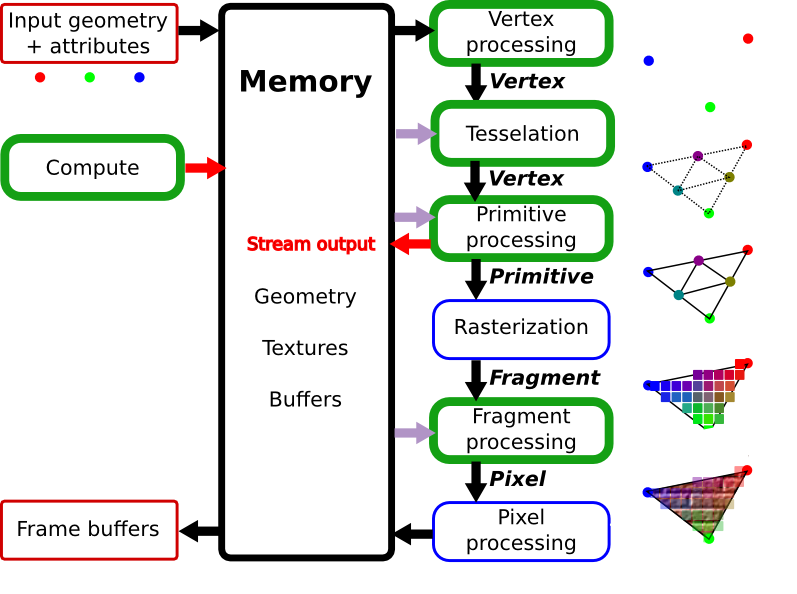
\includegraphics[width=\textwidth]{imagenes/pipeline-v4.png}
\caption{Pipeline programable de graficos de OpenGL 4.0. En verde las partes donde el usuario puede intervenir de forma directa}
\end{figure}

A partir de estos conceptos podemos definir los objetivos de nuestro trabajo como el de la creación de un algoritmo que a partir de la información que se utiliza para definir la profundidad de cada fragmento en la fase de rasterización pueda detectar y encontrar una convexidad concreta
percibida a partir del punto del punto de vista que nos da la camara. Y la creación de un Shader que nos permita transformar las primitivas que pertenecen a esa convexidad para poder moverlas en dirección a un plano definido por la linea de visión de la cara en el cual se encuentra el fin de la convexidad.

\section{Los Shaders y el lenguaje GLSL}

\subsection{Definición y consideraciones sobre los Shaders}

Antes de continuar describiendo el proyecto es interesante que paremos a introducir uno de los puntos claves del mismo.

Los Shaders son como hemos definido antes programas diseñados para ejecutarse en la unidad grafica del ordenador. Sin embargo esta definicion aunque correcta en la actualidad merece cierta matización. La primera vez que se acuño el termino Shader fue a finales de los años ochenta, fue acuñado por Pixar para el desarrollo de su interfaz RenderMan 3.0 y en su momento eran solo pequeños programas que se ejecutaban en el procesador
y permitian cierto control del renderizado de los objetos tridimensionales. Sin embargo con la evolución de las tarjetas graficas esta forma de trabajar se volvio popular, principalmente por razones de rendimiento. 

A medida que el campo de los graficos de ordenador fue evolucionando y tuvimos necesidad de renderizar escenas cada vez mas realistas y complejas nos dimos cuenta que el trabajar el renderizado en el procesador no era una solución eficiente. Esto se debe a que cuando estamos renderizando podemos romper la tarea en hacer los calculos pertinentes para cada vertice. Los cuales a nivel de cada vertice
no son calculos excesivamente complejos, sin embargo si son una gran cantidad de calculos. Actualmente los ordenadores modernos tienen grupos de microprocesadores que se dividen todas las tareas que el ordenador tiene que ir resolviendo y trabajan en ellas de forma paralela. Supongamos una pantalla de 800x600 renderizando pixel por pixel una aplicación grafica. Si este fuera el caso, en cada frame de la aplicación
tenemos que procesar un total de 480.000 pixeles por cada frame que estemos ejecutando la aplicación, si quisieramos mantener esa aplicación a un rendimiento de 60 frames por segundo tendriamos que estar procesando un total de 28.800.000 pixeles por segundo y en pantallas modernas de mayor resolución este numero solo aumenta. Al punto en que sería capaz de sobrecargar un procesador. \cite{thebookofshadersBookShaders}

La forma de solventar es esto es utilizar la programación paralela que ofrecen las graficas por su arquitectura. Diseñadas originalmente para acelerar los calculos necesarios para los graficos por ordenador una tarjeta grafica esta compuesta por un conjunto de multiples pequeños procesadores capaz de trabajar de forma paralela con cada pixel de la pantalla. De forma que en vez de ser el procesador general del computador el que trabaja con todos los pixeles repartiendoselos de forma secuencial todos ellos son procesados de forma paralela por la grafica. Ademas de ello 
muchas graficas implementan circuitos capaces de realizar ciertas operaciones matematicas complejas propias del procesado de graficos. Esto provoca una aceleración con respecto a realizar estas operaciones por software.

Esto aunque es eficiente nos genera una serie de limitaciones que hace que el uso de Shaders presente algunas dificultades. Por ejemplo como todas las operaciones estan ocurriendo en paralelo cada pequeño procesador es independiente de todos sus vecinos. Por tanto mientras estas procesando un dato es imposible consultar o modificar el resultado de sus datos vecinos. Ademas de ello la GPU se mantiene siempre ocupada, y por tanto es imposible para un procesador saber que estaba haciendo en el momento anterior. Por tanto no mantienen memoria

\subsection{Especificación del lenguaje GLSL}

El estandar OpenGL introdujo los shaders con la versión 2.0 en el 2004. Junto con el lenguaje GLSL, el cual ademas de ser un lenguaje similar a C ofrecia una serie de funciones y utilidades que permitian facilitar el desarrollo de los Shaders. No es el unico lenguaje para la especifiación de Shaders que existe, encontrando alternativas como MSL O Metal Shading Language utilizado por la especificación de graficos Metal, RSL que es el lenguaje que utiliza la especificación de Renderman creada por pixar. Podemos hacer que OpenGL soporte otros lenguajes de Shaders mediante extensiones,
 pero por defecto OpenGL soporta GLSL.

La forma en la que se compila un programa en GLSL hace que tengamos que usar una terminologia especifica cuando nos queramos referir a el. En GLSL un shader es una serie de strings compilados que afectan a una fase del pipeline de graficos. Mientras que un programa es un conjunto de estos shaders que cubre multiples fases del pipeline. Ademas de ello nos ofrece capacidades como los uniformes, variables nombradas que podemos utilizar en los shaders que podemos enviar desde CPU. Ademas de una lista de variables predefinidas con valores utiles. Explicaremos individualmente las especificaciones del lenguaje
que utilicemos en la sección de desarrollo a medida que vayamos necesitandolas.

Otro elemento util que merece la pena explicar son los Samplers, que son conjuntos de datos que la grafica puede leer. El uso mas comun de estos Samplers es para las texturas



\section{Motivaciones}

El proposito por el que se ha creado este proyecto es el de crear una herramienta que permita a los artistas modificar las convexidades de diferentes modelos 3D. Aunque la idea especifica del proyecto es imitar el estilo de Pablo Gargallo la herramienta que estamos desarrollando se diferencia a si misma de los ultimos
avances en transferencia de estilo en tanto y cuanto estos ultimos no permiten la agencia de un usuario humano y utilizan tecnicas avanzadas de Aprendizaje profundo para realizar esta transformación de forma automática, con las limitaciones que estas implican, como la no explicabilidad de lo que esta sucediendo. Nuestro enfoque en cambio es mas similar al de una herramienta de modelado. En la cual el artista podra
controlar que convexidad esta modificando y el grado de modificación que quiere efectuar mientras observa en tiempo real los efectos de sus acciones.


Este proyecto es software libre, y está liberado con la licencia \cite{gplv3}.